\section{Arming Logic}

The control logic that the pad server uses to govern which actuation and arming commands are valid at any given time
are based on the arming state in Figure 13.

\begin{figure}[H]
    \centering
    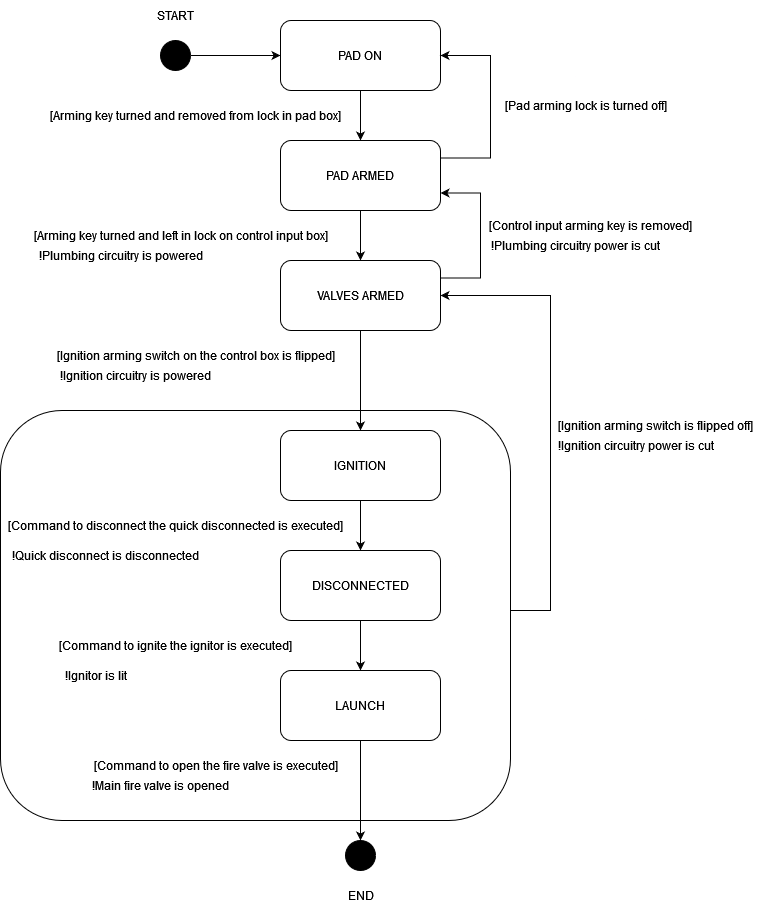
\includegraphics[width=4in]{./assets/Hybrid_Control_FSM.png}
    \caption{Finite state machine for arming control}
    \label{fig:logging-fsm}
\end{figure}

\begin{table}[H]
    \centering
    \begin{tabular}{| c | c | p{2in} |}
        \hline
        State               & Available actuator IDs (inclusive) & Description                                        \\
        \hline
        ARMED\_PAD          & None                               &                                                    \\
        \hline
        ARMED\_VALVES       & 1-12                               & All solenoid valves (XV-1 to XV-12)                \\
        \hline
        ARMED\_IGNITION     & 1-13                               & All solenoid valves and the quick disconnect       \\
        \hline
        ARMED\_DISCONNECTED & 1-14                               & All solenoid valves, quick disconnect and igniter  \\
        \hline
        ARMED\_LAUNCH       & 0-14                               & All solenoid valves, quick disconnect, igniter and
        main fire valve                                                                                               \\
        \hline
    \end{tabular}
    \caption{Available actuators for each arming state}
    \label{tbl:available-actuators}
\end{table}

The quick disconnect is an actuator which upon being switched "on", forcibly disconnects the ground systems plumbing
from the oxidizer tank on board the rocket. This operation cannot be reversed.

The igniter is a small piece of solid fuel with nichrome wires running through it. Once it is turned "on", high current
is sent through the nichrome wires, igniting a flame underneath the fire valve. This action cannot be reversed.

The main fire valve is a single valve that when opened, allows the oxidizer to flow out of the oxidizer tank on the
rocket and into the combustion chamber. It will flow out of the nozzle on the combustion chamber on to the lit igniter,
initiating lift-off. This action \textit{obviously} cannot be reversed!
